% !TeX root = ../../main.tex
\subsection{Phân tích OLAP trên Data Mart}\label{sec:olap}

Theo mô hình ROLAP đã chọn (mục~\ref{sec:kientruc}), khối dữ liệu chính là bảng fact \code{fact\_sales} cùng các bảng chiều, và mỗi phép toán OLAP là một truy vấn SQL dùng \code{GROUP BY}, \code{ROLLUP} hoặc \code{CUBE}. Tập tin \code{50\_olap\_queries.sql} có 14 truy vấn, mỗi truy vấn trả lời một nhu cầu ở Bảng~\ref{tab:quyetdinh}. Hai quy ước được áp dụng cho mọi truy vấn: thước đo theo đơn hàng (thời gian giao, cờ trễ, điểm đánh giá) luôn lấy từ view \code{dm.v\_order} để mỗi đơn chỉ được tính một lần (mục~\ref{sec:dodo}), và doanh thu không tính các đơn ở trạng thái \code{canceled} hay \code{unavailable}.

\subsubsection{Roll-up}

Phép roll-up tổng hợp doanh thu theo phân cấp Tháng $\rightarrow$ Quý $\rightarrow$ Năm. Chỉ với một câu lệnh \code{GROUP BY ROLLUP (year, quarter, month)}, PostgreSQL trả về cùng lúc dòng chi tiết theo tháng, dòng tổng theo quý, theo năm và dòng tổng toàn bộ.

\begin{lstlisting}[style=SQLStyle]
SELECT d.year, d.quarter, d.month,
       SUM(f.price) AS revenue, COUNT(DISTINCT f.order_id) AS orders
FROM dm.fact_sales f JOIN dm.dim_date d ON d.date_key = f.purchase_date_key
WHERE f.order_status NOT IN ('canceled', 'unavailable')
GROUP BY ROLLUP (d.year, d.quarter, d.month);
\end{lstlisting}

Bảng~\ref{tab:rollup} là kết quả ở mức quý và năm; Hình~\ref{fig:rollupthang} vẽ lại mức tháng trong giai đoạn 01/2017-08/2018.

\begin{table}[H]
\centering
\small\setstretch{1.1}
\caption{Kết quả roll-up doanh thu theo quý và năm}
\label{tab:rollup}
\begin{tabularx}{\linewidth}{|P{2.4cm}|>{\raggedleft\arraybackslash}X|>{\raggedleft\arraybackslash}X|>{\raggedleft\arraybackslash}X|}
\hline
\textbf{Kỳ} & \textbf{Doanh thu (BRL)} & \textbf{Số đơn} & \textbf{Giá trị đơn TB (BRL)}\\ \hline
Quý 1/2017 & 733.398,94 & 5.122 & 143,19\\ \hline
Quý 2/2017 & 1.286.918,78 & 9.222 & 139,55\\ \hline
Quý 3/2017 & 1.681.949,00 & 12.445 & 135,15\\ \hline
Quý 4/2017 & 2.406.225,55 & 17.586 & 136,83\\ \hline
\textbf{Năm 2017} & \textbf{6.108.492,27} & \textbf{44.375} & \textbf{137,66}\\ \hline
Quý 1/2018 & 2.764.402,78 & 20.979 & 131,77\\ \hline
Quý 2/2018 & 2.849.730,26 & 19.897 & 143,22\\ \hline
Quý 3/2018 (07-09/2018) & 1.727.049,37 & 12.655 & 136,47\\ \hline
\textbf{Năm 2018} & \textbf{7.341.182,41} & \textbf{53.531} & \textbf{137,14}\\ \hline
\textbf{Toàn bộ (2016-2018)} & \textbf{13.494.400,74} & \textbf{98.199} & \textbf{137,42}\\ \hline
\end{tabularx}
\end{table}

\begin{figure}[H]
\centering
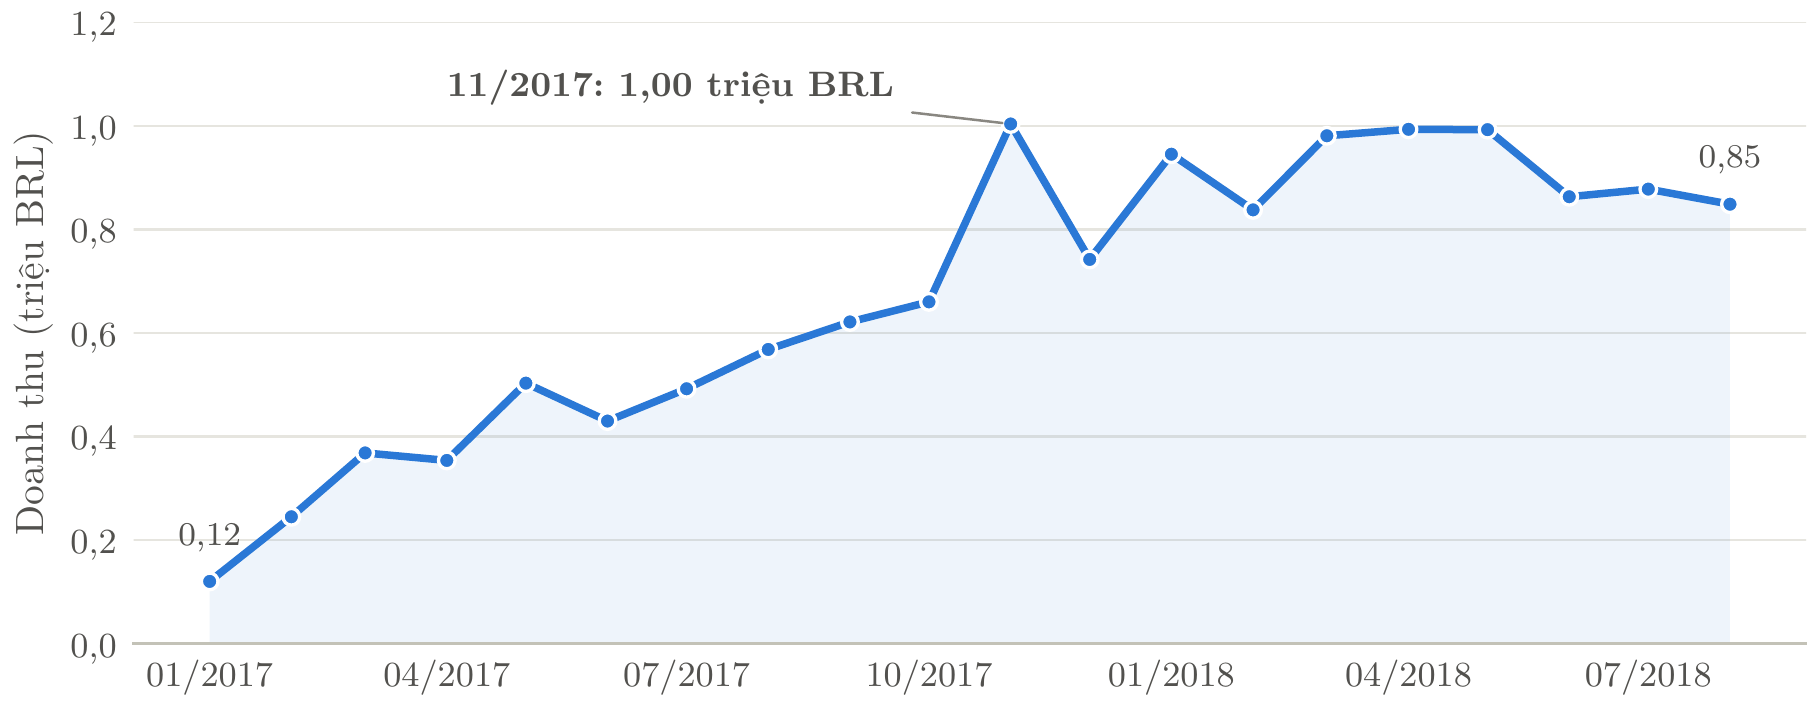
\includegraphics{Pictures/fig-olap-rollup-thang.png}
\caption{Doanh thu hàng hóa theo tháng, giai đoạn 01/2017-08/2018 (mức tháng của phép roll-up)}
\label{fig:rollupthang}
\end{figure}

Doanh thu tăng đều qua từng quý của năm 2017 và lên đỉnh vào tháng 11/2017 với 1,00 triệu BRL, rồi giảm mạnh ở tháng 12. Sang năm 2018, doanh thu mỗi quý đứng quanh mức 2,8 triệu BRL; quý 3/2018 thấp hơn chỉ vì dữ liệu dừng ở tháng 08/2018. Giá trị đơn trung bình hầu như không đổi, khoảng 137 BRL, nên có thể nói tăng trưởng của sàn đến từ số đơn hàng chứ không phải từ việc khách mua đơn lớn hơn.

\subsubsection{Drill-down}

Phép drill-down đi ngược chiều roll-up: từ vùng xuống bang rồi xuống thành phố của khách hàng, ở đây để tìm nơi giao trễ nhiều. Bảng~\ref{tab:drilldown} là mức vùng kèm một vài bang tiêu biểu; Hình~\ref{fig:drilldown} là mức bang đầy đủ, mỗi thanh được tô theo vùng mà bang đó thuộc về.

\begin{table}[H]
\centering
\small\setstretch{1.1}
\caption{Drill-down tỷ lệ giao trễ từ vùng xuống bang}
\label{tab:drilldown}
\begin{tabularx}{\linewidth}{|P{3.0cm}|>{\raggedleft\arraybackslash}X|>{\raggedleft\arraybackslash}X|>{\raggedleft\arraybackslash}X|}
\hline
\textbf{Vùng / Bang} & \textbf{Số đơn đã giao} & \textbf{Tỷ lệ trễ} & \textbf{Thời gian giao TB (ngày)}\\ \hline
Sudeste & 66.197 & 6,12\% & 10,8\\ \hline
\quad RJ & 12.351 & 12,11\% & 15,3\\ \hline
\quad SP & 40.499 & 4,49\% & 8,8\\ \hline
Sul & 13.812 & 5,90\% & 14,0\\ \hline
Centro-Oeste & 5.619 & 6,50\% & 15,0\\ \hline
Nordeste & 9.045 & 12,71\% & 20,0\\ \hline
\quad AL & 397 & 21,41\% & 24,5\\ \hline
\quad MA & 720 & 17,36\% & 21,5\\ \hline
Norte & 1.797 & 8,57\% & 22,6\\ \hline
\textbf{Toàn quốc} & \textbf{96.470} & \textbf{6,77\%} & \textbf{12,6}\\ \hline
\end{tabularx}
\end{table}

\begin{figure}[H]
\centering
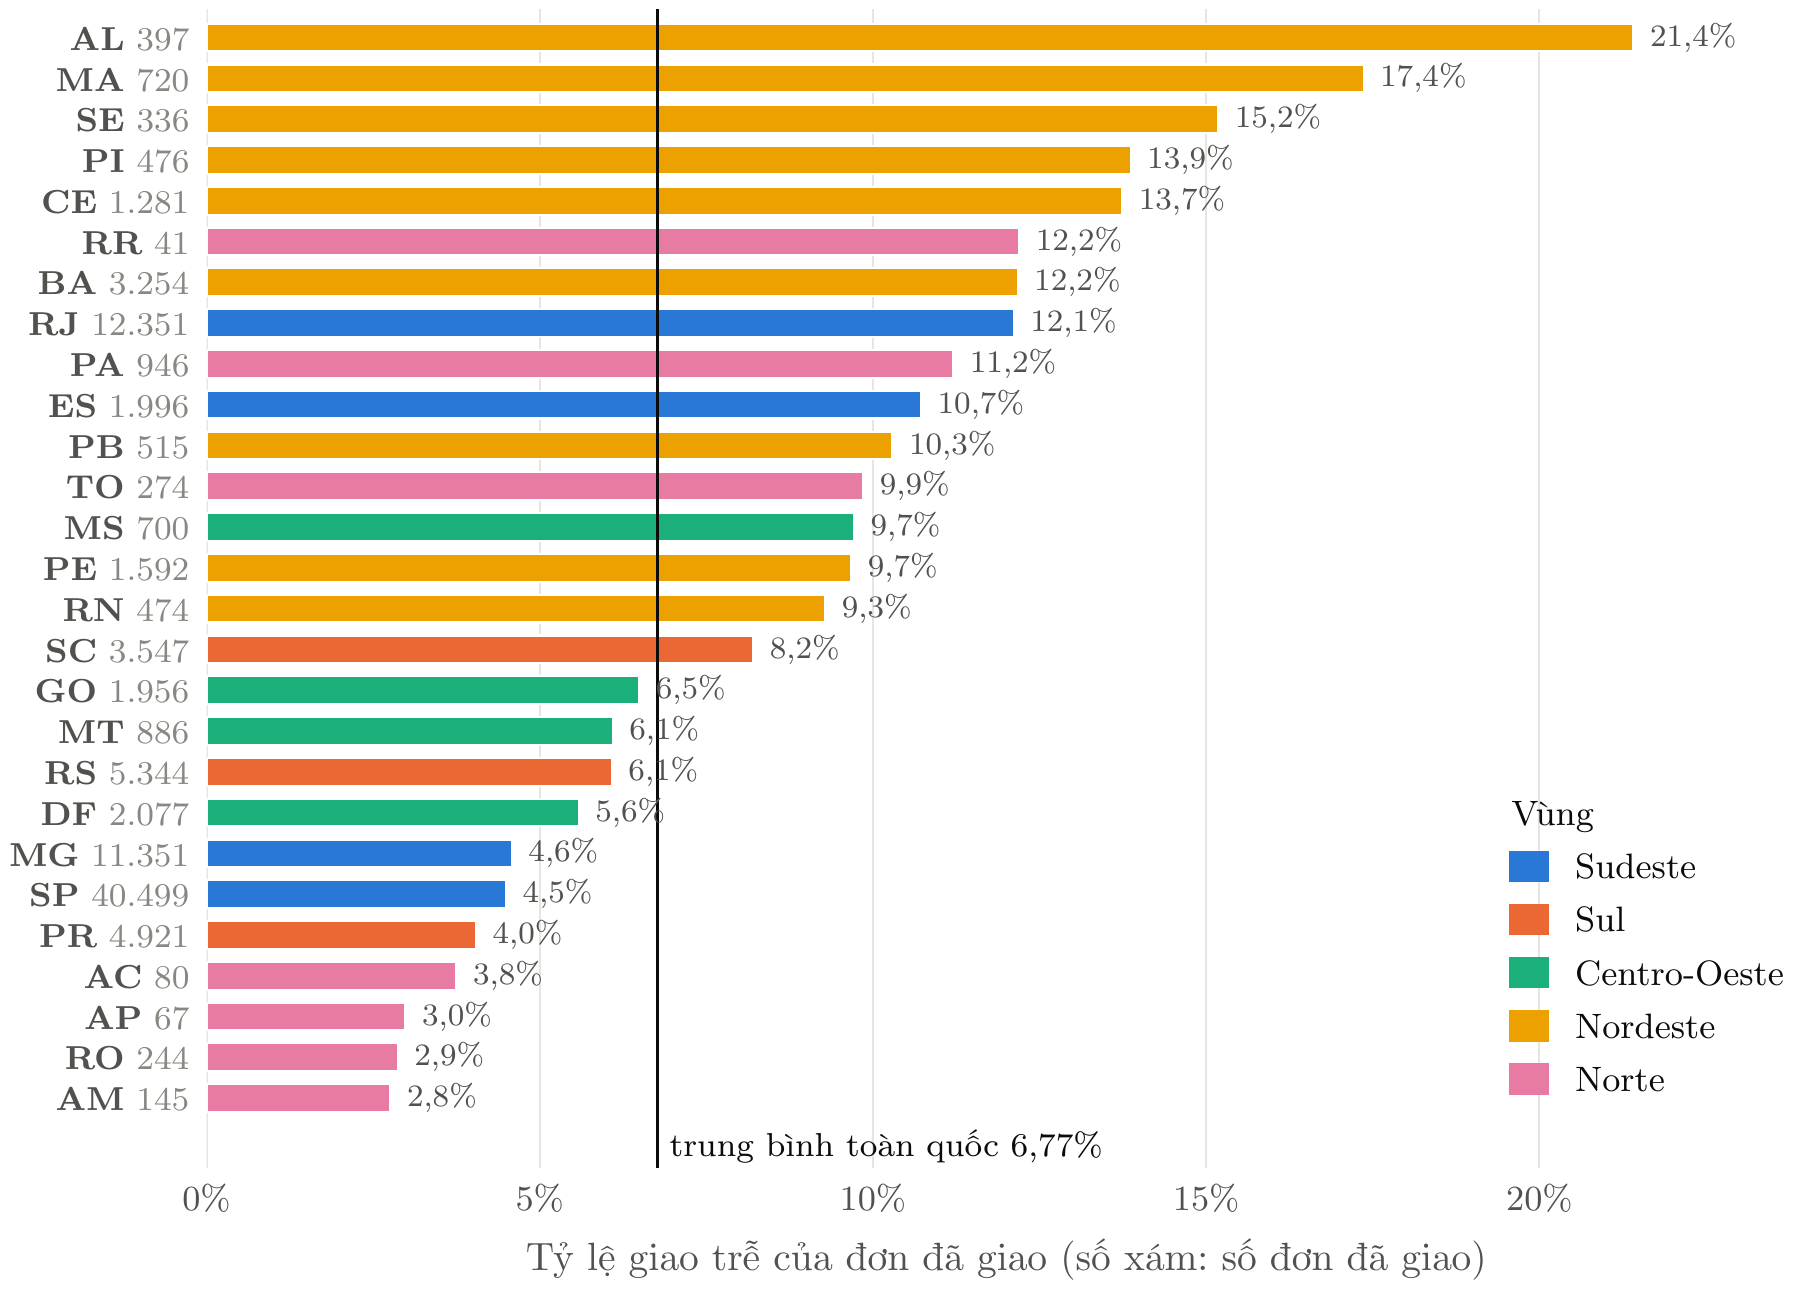
\includegraphics{Pictures/fig-olap-drilldown-bang.png}
\caption{Tỷ lệ giao trễ theo bang của khách hàng, tô màu theo vùng (mức bang của phép drill-down)}
\label{fig:drilldown}
\end{figure}

Ở mức vùng, Nordeste có tỷ lệ trễ 12,71\%, gần gấp đôi trung bình toàn quốc, và Hình~\ref{fig:drilldown} cho thấy gần như mọi bang của Nordeste đều nằm trên đường trung bình. Điều bất ngờ hơn chỉ lộ ra khi drill-down: Sudeste, vùng có tỷ lệ trễ thấp, lại chứa bang RJ với 12,11\%, gần gấp ba bang SP bên cạnh. Đi tiếp xuống thành phố của RJ, \code{sao goncalo} trễ 21,50\% trên 386 đơn, còn thành phố \code{rio de janeiro} là 10,72\% trên 6.597 đơn. Nếu chỉ nhìn ở mức vùng, nhà quản lý sẽ bỏ qua một điểm nóng giao trễ ở nơi có nhiều đơn hàng thứ hai cả nước.

Hình~\ref{fig:drilldown} cũng nhắc lại giới hạn đã nêu ở mục~\ref{sec:quanhe}: các bang nhỏ như RR (41 đơn) hay AP (67 đơn) có quá ít đơn để tỷ lệ trễ của chúng đáng tin.

\subsubsection{Slice và Dice}

Phép slice cố định một giá trị trên một chiều; ở đây là năm 2018 trên chiều thời gian, xem doanh thu theo vùng (Bảng~\ref{tab:slice}). Phép dice chọn một tập giá trị trên nhiều chiều cùng lúc; ở đây là quý 4/2017, ba bang SP, RJ, MG và năm ngành hàng có doanh thu cao nhất năm 2017 (Hình~\ref{fig:dice}).

\begin{table}[H]
\centering
\small\setstretch{1.1}
\caption{Kết quả slice năm 2018: doanh thu theo vùng}
\label{tab:slice}
\begin{tabularx}{\linewidth}{|P{3.8cm}|>{\raggedleft\arraybackslash}X|>{\raggedleft\arraybackslash}X|>{\raggedleft\arraybackslash}X|}
\hline
\textbf{Vùng} & \textbf{Doanh thu (BRL)} & \textbf{Số đơn} & \textbf{Tỷ trọng doanh thu}\\ \hline
Sudeste & 4.866.163,13 & 37.301 & 66,3\%\\ \hline
Sul & 1.047.635,66 & 7.394 & 14,3\%\\ \hline
Nordeste & 804.697,84 & 4.801 & 11,0\%\\ \hline
Centro-Oeste & 458.089,53 & 3.152 & 6,2\%\\ \hline
Norte & 164.596,25 & 883 & 2,2\%\\ \hline
\end{tabularx}
\end{table}

\begin{figure}[H]
\centering
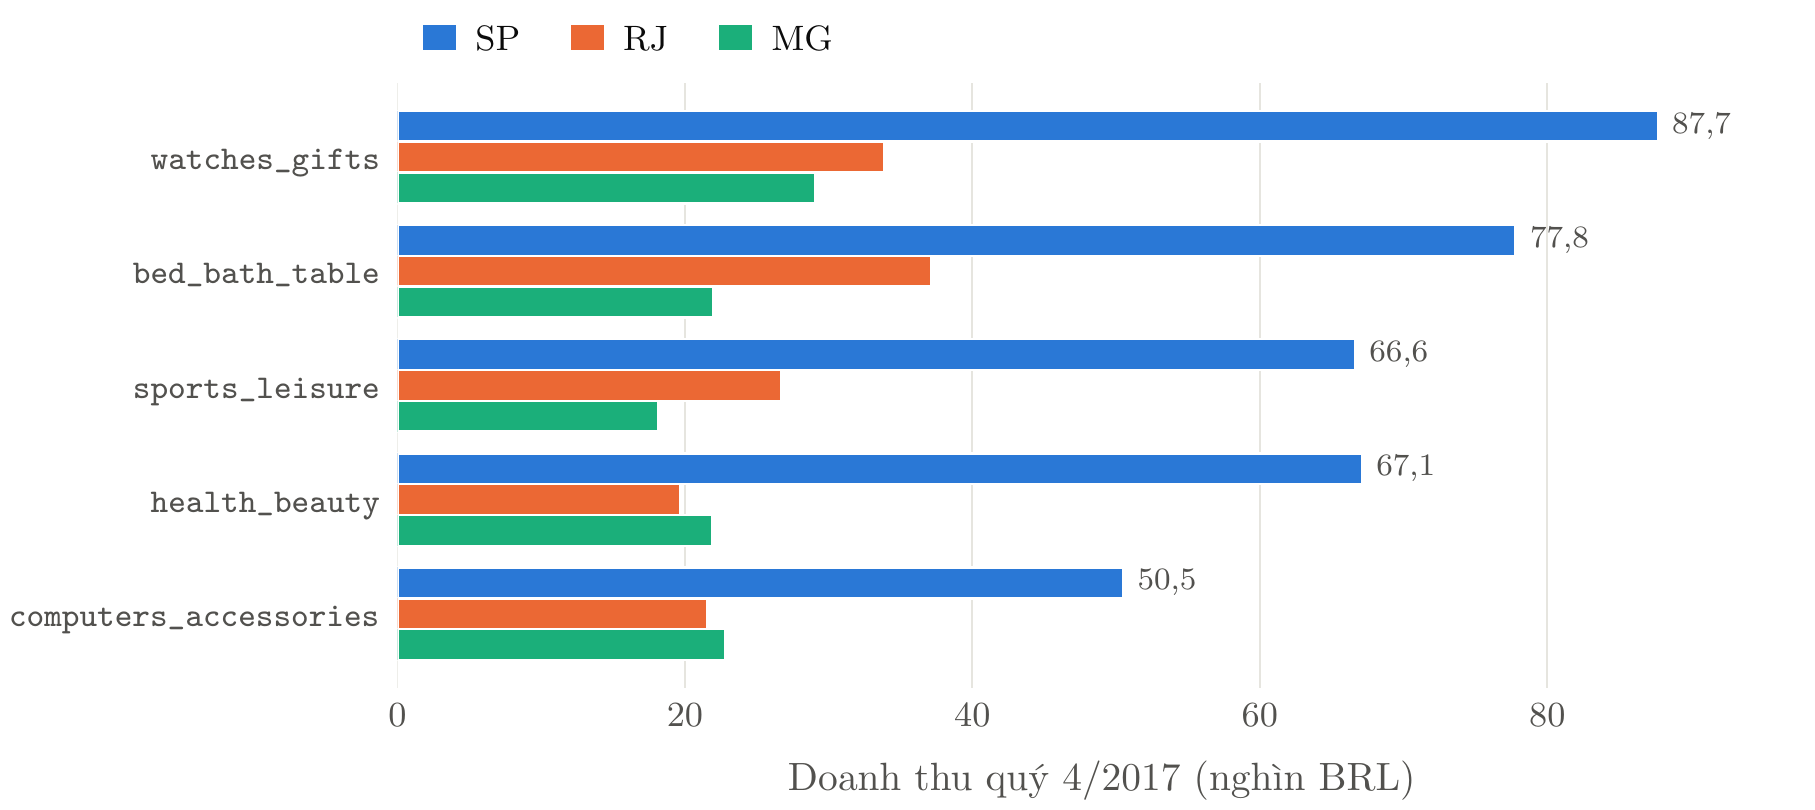
\includegraphics{Pictures/fig-olap-dice.png}
\caption{Kết quả dice: doanh thu quý 4/2017 của năm ngành hàng dẫn đầu năm 2017 tại các bang SP, RJ và MG}
\label{fig:dice}
\end{figure}

Năm 2018, riêng vùng Sudeste đã chiếm hai phần ba doanh thu. Trong mùa cao điểm quý 4/2017, SP dẫn đầu mọi ngành hàng như dự đoán, nhưng thứ tự ngành hàng thay đổi theo bang: \code{watches\_gifts} đứng đầu ở SP (87.690,54 BRL) và MG, trong khi ở RJ ngành bán chạy nhất là \code{bed\_bath\_table} (37.163,75 BRL). Một chương trình khuyến mãi chung cho cả ba bang vì vậy sẽ không tối ưu bằng chương trình riêng cho từng bang.

\subsubsection{Pivot}

Phép pivot xoay chiều vùng từ dòng sang cột để so điểm đánh giá của từng ngành hàng giữa các vùng. Trong SQL, phép xoay được viết bằng hàm tổng hợp có điều kiện \code{AVG(...) FILTER (WHERE region = ...)}, mỗi vùng một cột. Hình~\ref{fig:pivot} là kết quả cho mười ngành hàng có nhiều đơn nhất, sắp theo điểm trung bình chung tăng dần, từ 3,97 của \code{bed\_bath\_table} đến 4,20 của \code{toys}.

\begin{figure}[H]
\centering
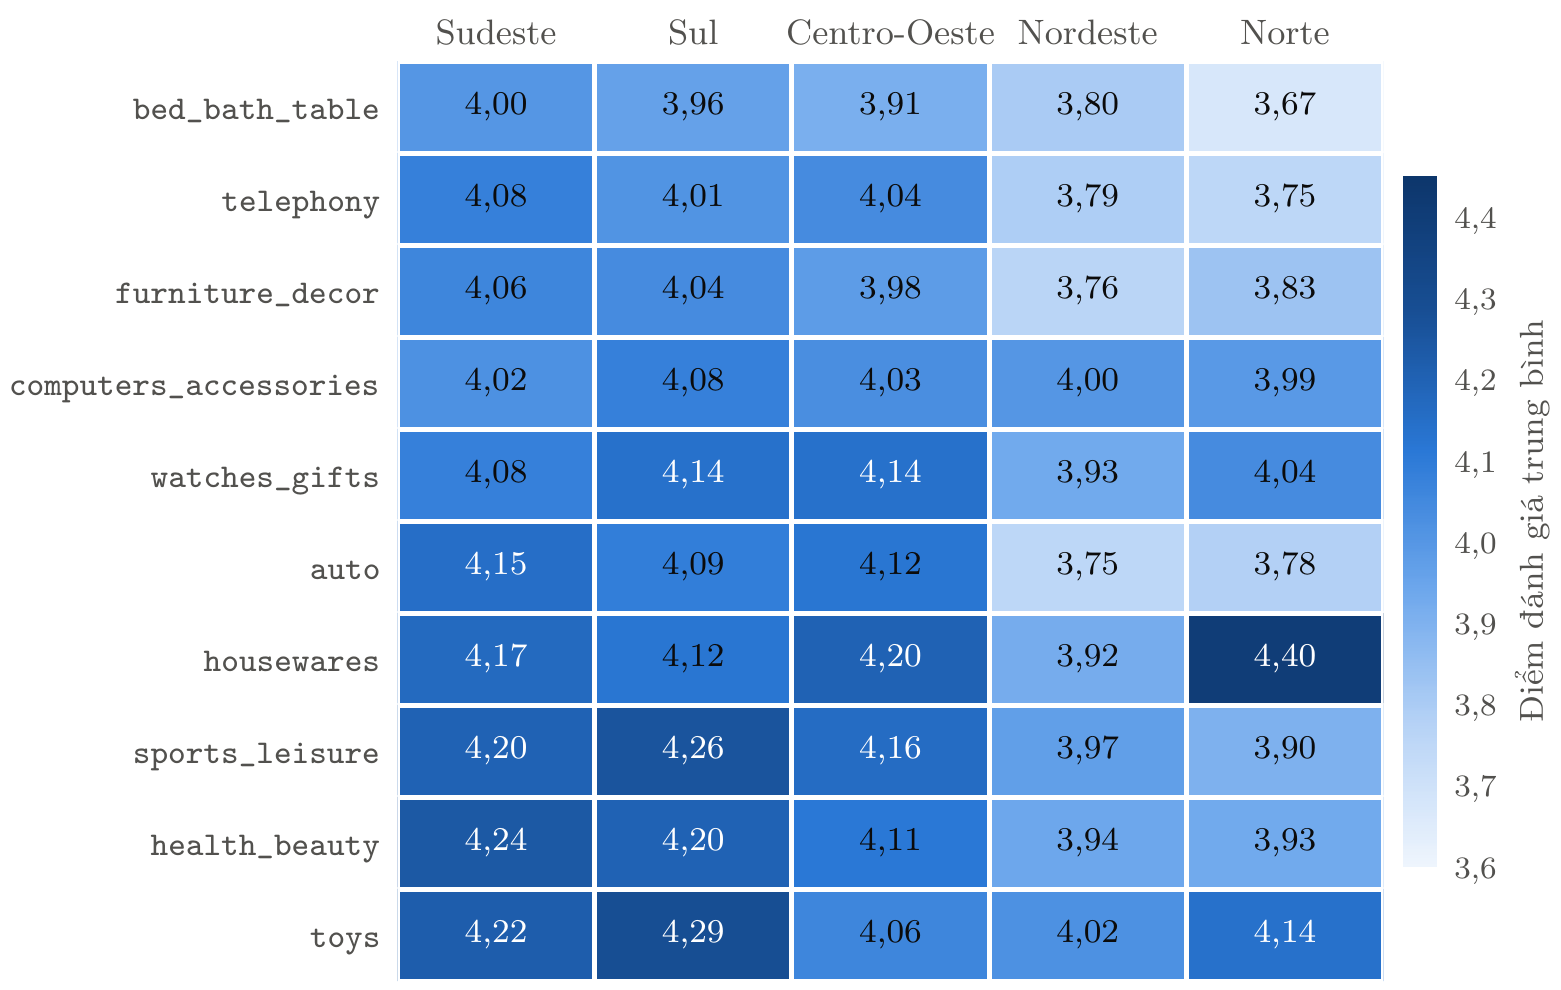
\includegraphics{Pictures/fig-olap-pivot.png}
\caption{Kết quả pivot: điểm đánh giá trung bình theo ngành hàng (dòng) và vùng của khách hàng (cột); màu càng đậm điểm càng cao}
\label{fig:pivot}
\end{figure}

Hai cột Nordeste và Norte nhạt hơn hẳn ba cột còn lại ở hầu hết các ngành hàng. Đây cũng là hai vùng có thời gian giao lâu nhất (Bảng~\ref{tab:drilldown}), một dấu hiệu nữa cho thấy điểm đánh giá gắn chặt với chất lượng giao hàng. Ô nổi bật duy nhất là \code{housewares} ở Norte (4,40), nhưng ô này chỉ dựa trên khoảng 60 đơn nên không đủ để kết luận.

\subsubsection{Các truy vấn phân tích nghiệp vụ}\label{sec:olapnghiepvu}

Ngoài năm phép toán cơ bản, thư viện truy vấn còn trả lời trực tiếp các câu hỏi của từng nhóm người dùng ở Bảng~\ref{tab:quyetdinh}.

\paragraph{Giao trễ và mức độ hài lòng}
Câu hỏi đầu tiên là giao trễ ảnh hưởng đến điểm đánh giá nhiều đến đâu. Trên 95.824 đơn có cả trạng thái giao hàng lẫn đánh giá, đơn đúng hạn được trung bình 4,29 điểm, còn đơn trễ chỉ 2,27 điểm. Hình~\ref{fig:trevadanhgia} cho thấy rõ hơn: hơn một nửa (53,8\%) đơn trễ bị chấm 1 sao, trong khi ở nhóm đúng hạn con số này chỉ là 6,6\%. Tỷ lệ 1-2 sao tăng từ 9,3\% lên 62,4\%. Với bộ phận chăm sóc khách hàng, điều này có nghĩa là giảm giao trễ là cách trực tiếp nhất để giảm đánh giá xấu; đây cũng là lý do thành phần hệ hỗ trợ quyết định của đề tài tập trung vào giao trễ.

\begin{figure}[H]
\centering
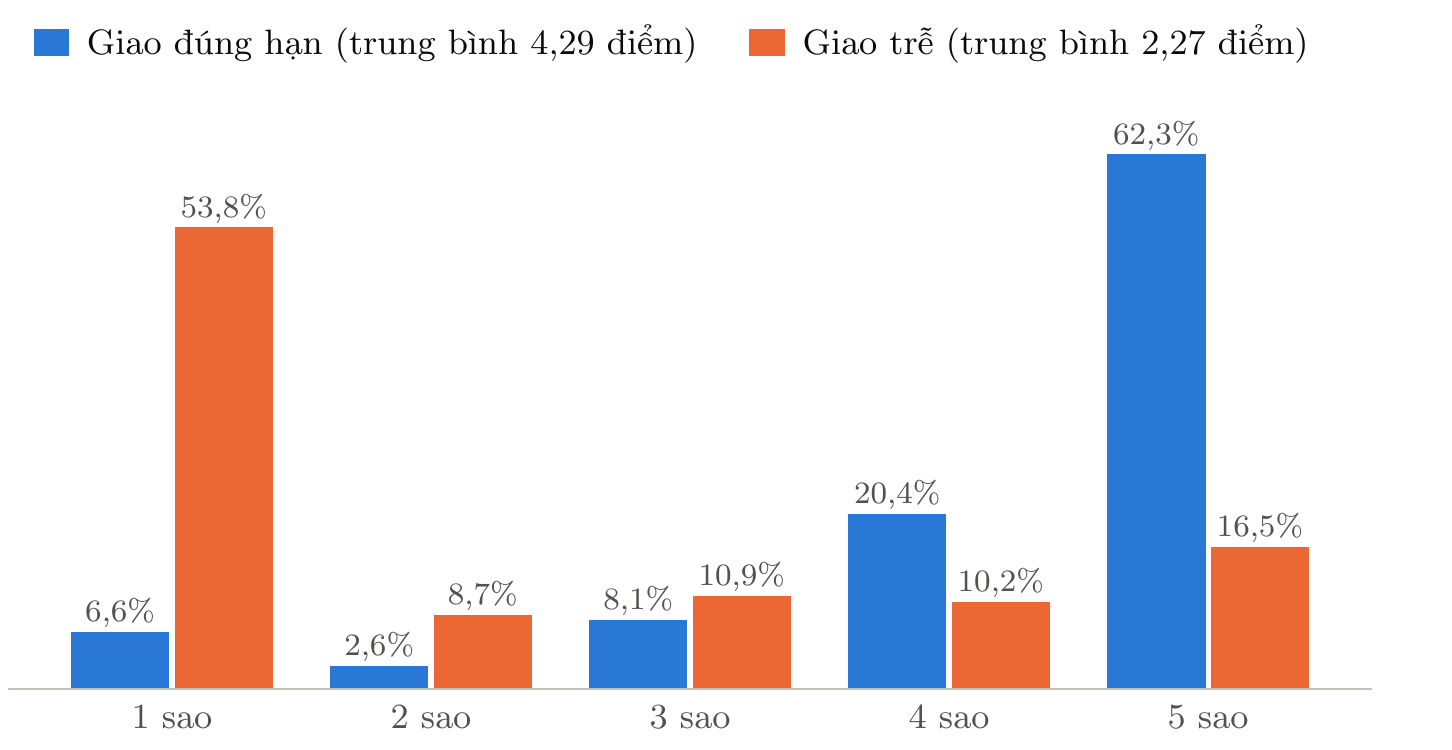
\includegraphics{Pictures/fig-tre-va-danh-gia.png}
\caption{Phân bố điểm đánh giá của đơn giao đúng hạn và đơn giao trễ}
\label{fig:trevadanhgia}
\end{figure}

\paragraph{Thời gian từng công đoạn}
Hình~\ref{fig:congdoan} tách thời gian giao hàng của mỗi vùng thành ba công đoạn. Thời gian duyệt đơn (0,41-0,52 ngày) và thời gian người bán chuẩn bị hàng (2,74-2,93 ngày) gần như giống nhau ở mọi vùng. Toàn bộ chênh lệch nằm ở khâu vận chuyển: 7,55 ngày tới Sudeste, nhưng 16,64 ngày tới Nordeste và 19,24 ngày tới Norte. Nói cách khác, khách ở miền Bắc nhận hàng chậm không phải do người bán chậm mà do quãng đường vận chuyển; muốn cải thiện thì phải làm việc với đơn vị vận chuyển hoặc phát triển người bán ngay tại các vùng này.

\begin{figure}[H]
\centering
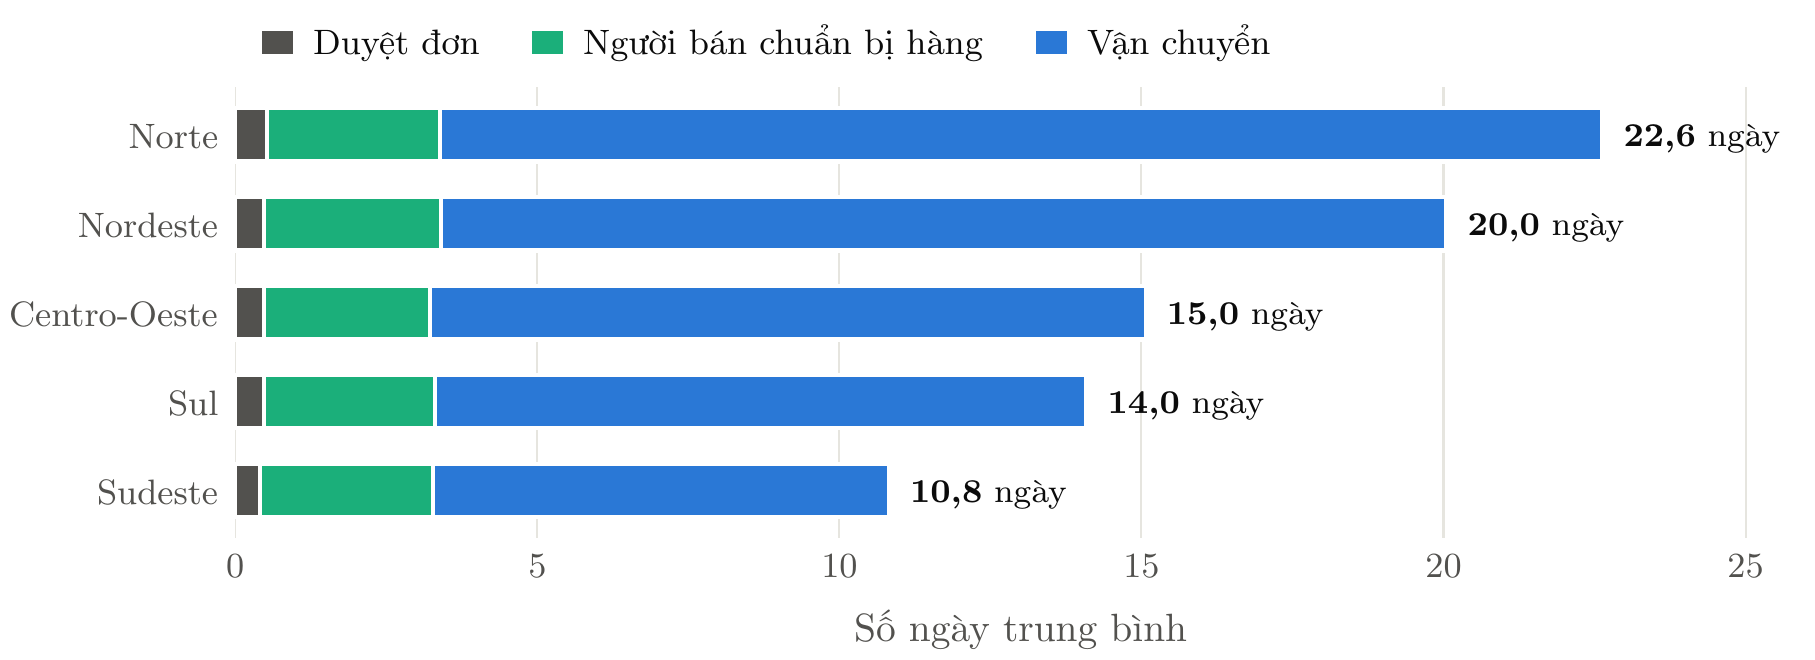
\includegraphics{Pictures/fig-olap-cong-doan.png}
\caption{Thời gian trung bình của từng công đoạn giao hàng theo vùng của khách hàng}
\label{fig:congdoan}
\end{figure}

\paragraph{Tuyến giao hàng}
Ma trận tuyến (Hình~\ref{fig:tuyengiao}) xét các lô hàng, tức cặp (đơn hàng, người bán), theo bang của người bán và bang của khách. Trong 50 tuyến có từ 200 lô trở lên, tỷ lệ trễ dao động từ 1,1\% (MG $\rightarrow$ PR) đến 23,7\% (SP $\rightarrow$ AL). Mọi tuyến từ SP đi các bang Nordeste đều trễ từ khoảng 10\% trở lên, cao nhất là đi AL, MA, PI và SE. Tuyến cần ưu tiên nhất với quản lý vận hành là SP $\rightarrow$ RJ: tỷ lệ trễ 14,0\% không phải cao nhất, nhưng tuyến này có tới 8.273 lô, nên đây là nơi cải thiện sẽ giảm được nhiều đơn trễ nhất.

\begin{figure}[H]
\centering
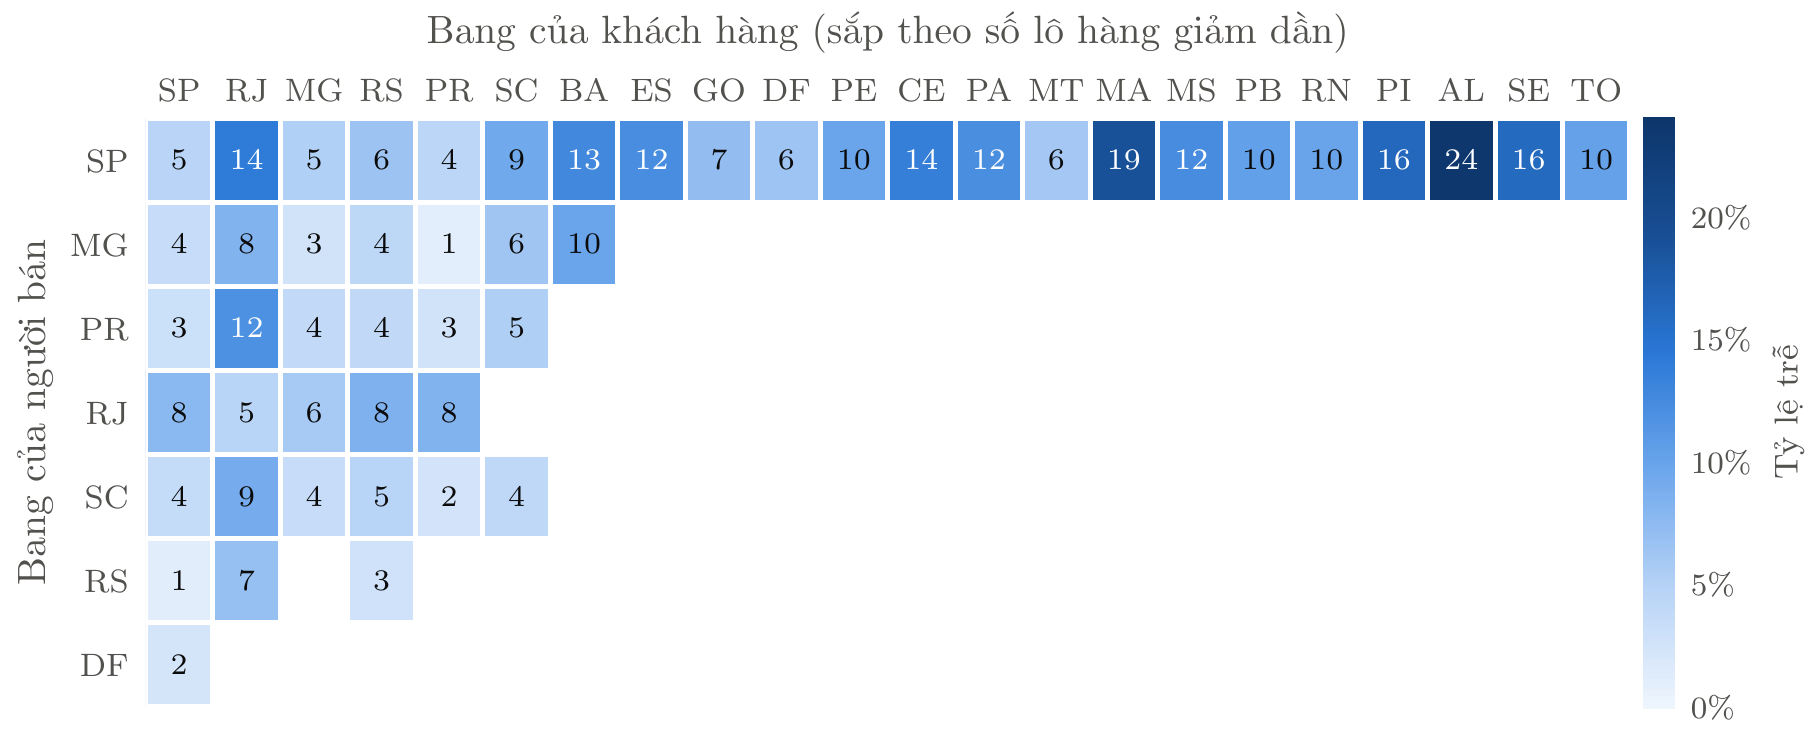
\includegraphics{Pictures/fig-olap-tuyen-giao.png}
\caption{Tỷ lệ giao trễ (\%) theo tuyến từ bang người bán đến bang khách hàng, chỉ gồm các tuyến có từ 200 lô hàng trở lên}
\label{fig:tuyengiao}
\end{figure}

\paragraph{Mùa cao điểm}
Ngày Black Friday 24/11/2017 có 1.166 đơn hàng, gấp hơn năm lần số đơn mỗi ngày của tuần trước đó (từ 146 đến 277 đơn). Hình~\ref{fig:blackfriday} cho thấy cái giá của đợt cao điểm này: các đơn đặt từ 24/11 đến 29/11/2017 có tỷ lệ trễ 17,3-20,9\%, gấp khoảng ba lần trung bình toàn kỳ, và phải sang tuần thứ hai của tháng 12 tỷ lệ trễ mới trở lại bình thường. Trước mùa cao điểm năm sau, sàn có cơ sở để nới ngày giao dự kiến hoặc tăng năng lực vận chuyển.

\begin{figure}[H]
\centering
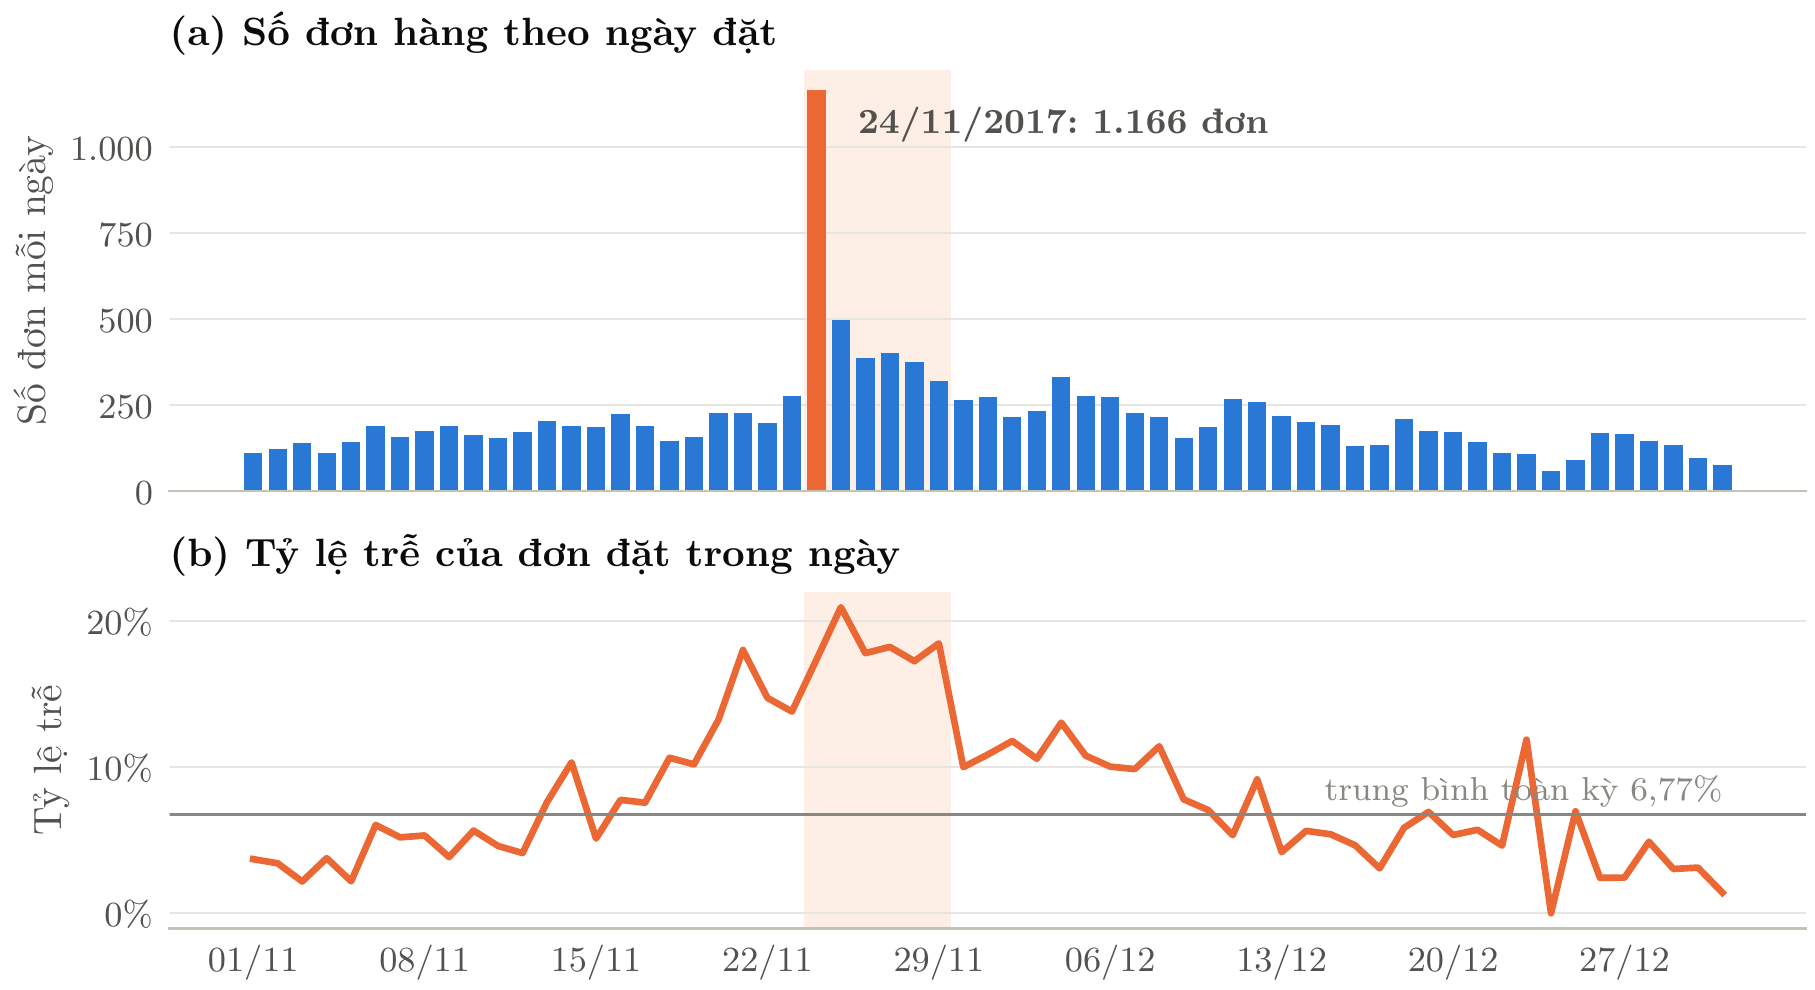
\includegraphics{Pictures/fig-olap-black-friday.png}
\caption{Số đơn hàng theo ngày (trên) và tỷ lệ giao trễ của đơn đặt trong ngày (dưới), tháng 11-12/2017; vùng tô xám là 24-29/11/2017}
\label{fig:blackfriday}
\end{figure}

\paragraph{Ngành hàng tăng trưởng}
So với cùng kỳ tháng 01-08/2017, doanh thu tháng 01-08/2018 của mọi ngành hàng lớn đều tăng, nhưng tốc độ rất khác nhau (Hình~\ref{fig:tangtruong}). \code{baby}, \code{watches\_gifts} và \code{health\_beauty} tăng hơn gấp ba, trong khi \code{cool\_stuff} gần như đứng yên (+8,9\%). Với ban điều hành, nhóm ngành tăng nhanh là ứng viên cho việc mở rộng danh mục người bán.

\begin{figure}[H]
\centering
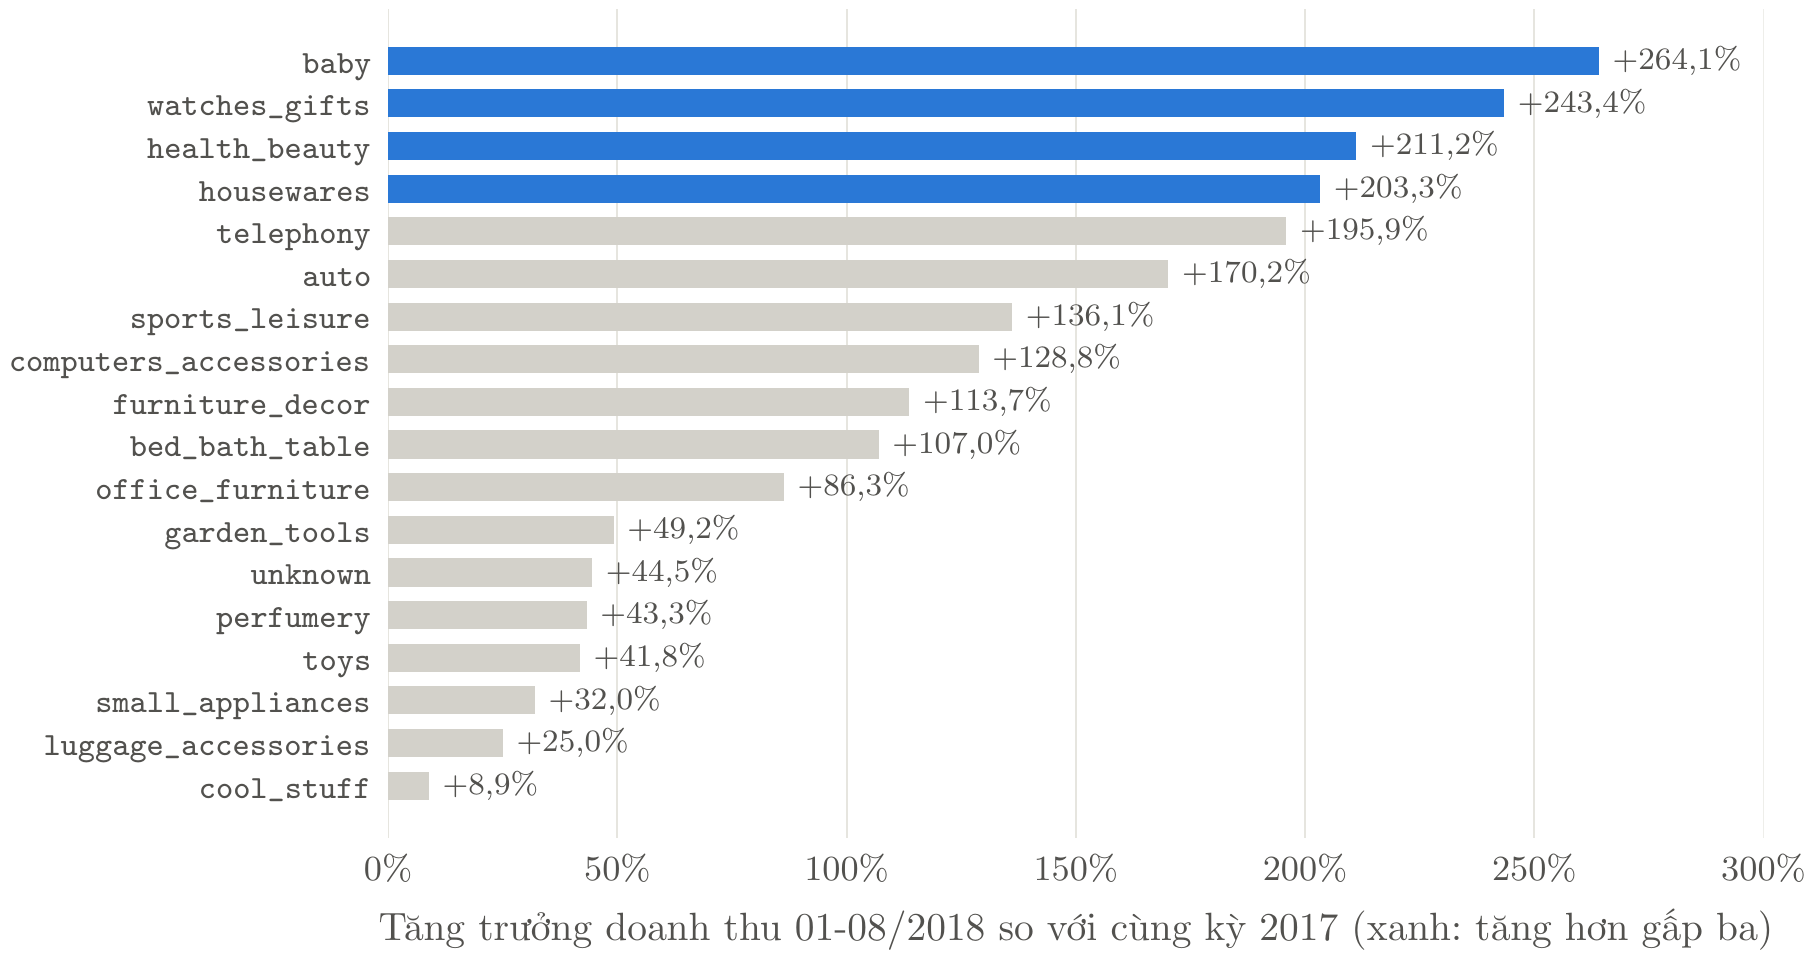
\includegraphics{Pictures/fig-olap-tang-truong-nganh.png}
\caption{Tăng trưởng doanh thu tháng 01-08/2018 so với cùng kỳ 2017 của các ngành hàng có doanh thu từ 50.000 BRL trong năm 2017}
\label{fig:tangtruong}
\end{figure}

\paragraph{Người bán}
Có 12 người bán thuộc nhóm 20\% doanh thu cao nhất nhưng có hơn 20\% đánh giá 1-2 sao. Người bán lớn nhất trong nhóm này có 973 đơn, doanh thu 186.570,05 BRL và 25,4\% đánh giá thấp; đây là kiểu người bán mà quản lý ngành hàng cần làm việc trước tiên, vì vừa quan trọng về doanh thu vừa đang làm giảm trải nghiệm của nhiều khách. Ở góc độ phân bố, Hình~\ref{fig:nguoibankhachhang} cho thấy SP chiếm 59,7\% người bán nhưng chỉ 41,9\% đơn hàng, còn RJ có 12,9\% đơn hàng nhưng chỉ 5,5\% người bán. Phần lớn đơn của RJ vì vậy phải đi liên bang từ SP, và điều này khớp với tỷ lệ trễ cao của tuyến SP $\rightarrow$ RJ ở trên.

\begin{figure}[H]
\centering
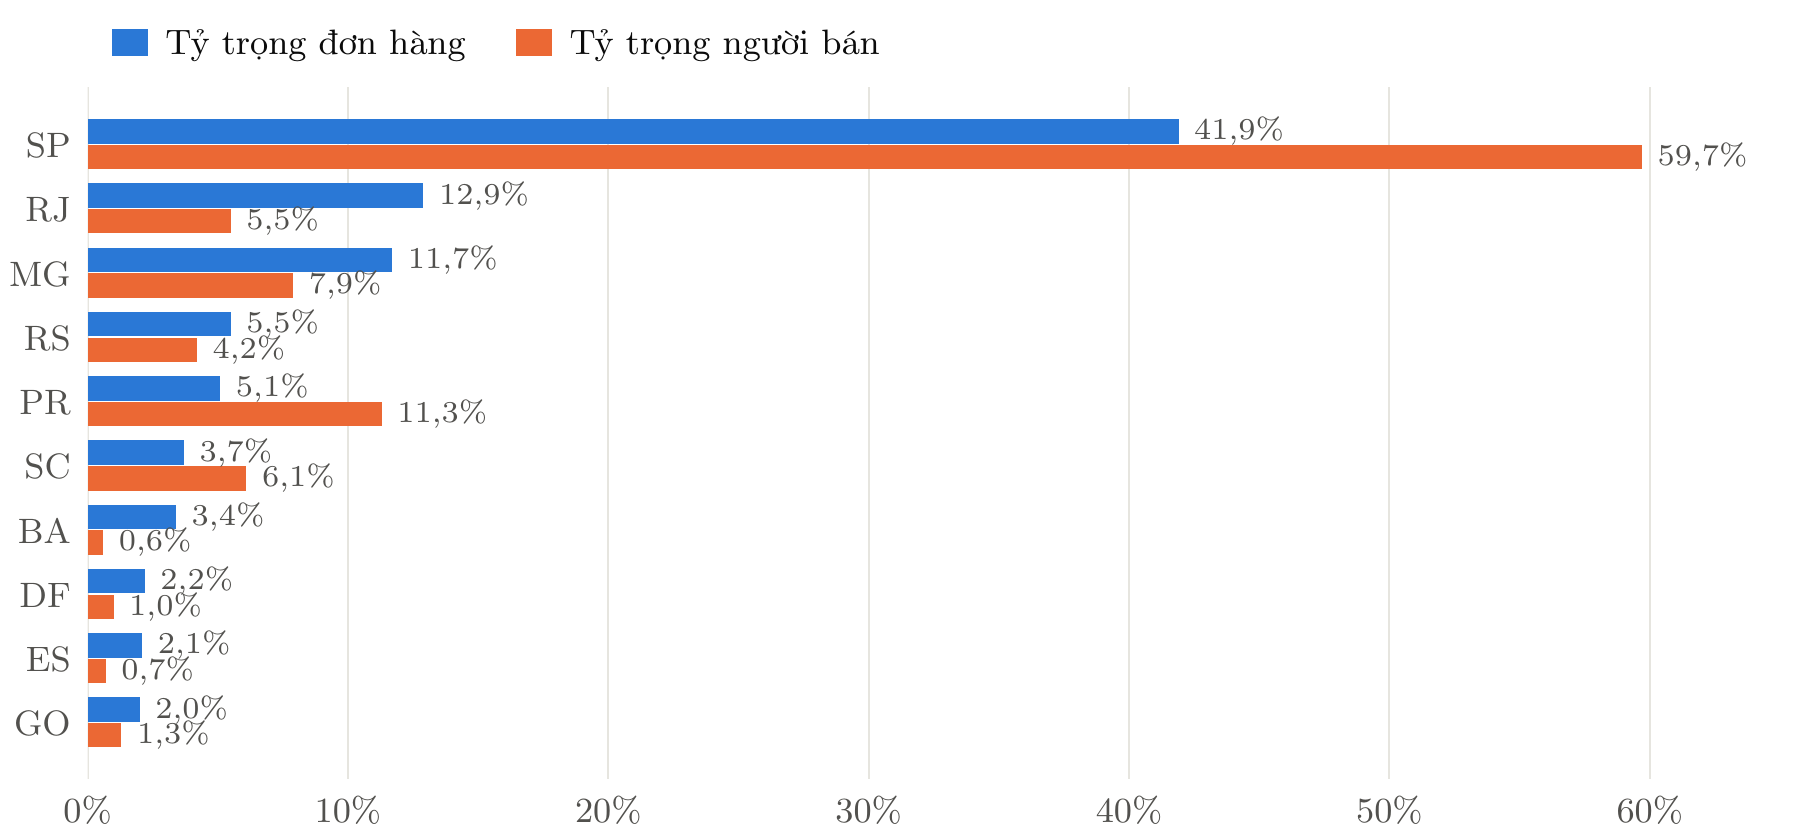
\includegraphics{Pictures/fig-olap-nguoi-ban-khach-hang.png}
\caption{Tỷ trọng người bán và tỷ trọng đơn hàng theo bang (10 bang có nhiều đơn hàng nhất)}
\label{fig:nguoibankhachhang}
\end{figure}

Đặt các kết quả này cạnh nhau sẽ ra một kết luận làm đầu vào cho phần hệ hỗ trợ quyết định: giao trễ là nguyên nhân chính làm giảm mức độ hài lòng, và giao trễ phụ thuộc rõ vào tuyến giao hàng, mùa vụ và người bán.

\subsubsection{Thời gian thực thi truy vấn}

Mỗi truy vấn được chạy năm lần bằng \code{EXPLAIN ANALYZE}, lấy trung vị thời gian thực thi trên máy chủ cơ sở dữ liệu (Bảng~\ref{tab:thoigiantruyvan}).

\begin{table}[H]
\centering
\small\setstretch{1.1}
\caption{Thời gian thực thi các truy vấn OLAP (trung vị của 5 lần chạy)}
\label{tab:thoigiantruyvan}
\begin{tabularx}{\linewidth}{|>{\raggedright\arraybackslash}X|P{2.0cm}|P{2.6cm}|}
\hline
\textbf{Truy vấn} & \textbf{Số dòng kết quả} & \textbf{Thời gian (ms)}\\ \hline
Roll-up doanh thu theo năm, quý, tháng & 37 & 545,6\\ \hline
Drill-down tỷ lệ trễ theo vùng, bang & 33 & 208,5\\ \hline
Drill-down tỷ lệ trễ theo thành phố của RJ & 4 & 100,3\\ \hline
Slice năm 2018 theo vùng & 5 & 219,0\\ \hline
Dice quý 4/2017 theo bang và ngành hàng & 15 & 230,1\\ \hline
Pivot điểm đánh giá theo ngành hàng và vùng & 10 & 454,9\\ \hline
Giao trễ và mức độ hài lòng & 2 & 74,6\\ \hline
Ma trận tuyến giao hàng & 50 & 311,8\\ \hline
Thời gian từng công đoạn theo vùng & 6 & 476,9\\ \hline
Người bán doanh thu cao, chất lượng thấp & 12 & 168,6\\ \hline
Phân bố người bán và đơn hàng theo bang & 27 & 179,8\\ \hline
Ngành hàng tăng trưởng & 18 & 57,7\\ \hline
CUBE vùng và năm & 24 & 717,3\\ \hline
Black Friday theo ngày & 15 & 93,5\\ \hline
\end{tabularx}
\end{table}

Truy vấn chậm nhất là CUBE theo vùng và năm, mất 0,72 giây, đủ nhanh để dashboard gọi trực tiếp. Kết quả này xác nhận nhận định ở mục~\ref{sec:luocdo}: với lượng dữ liệu hiện tại, các phép kết nối thêm của snowflake schema không làm chậm đáng kể, và chưa cần đến bảng tổng hợp lưu sẵn.
